% Created by tikzDevice version 0.12 on 2018-09-26 16:24:06
% !TEX encoding = UTF-8 Unicode
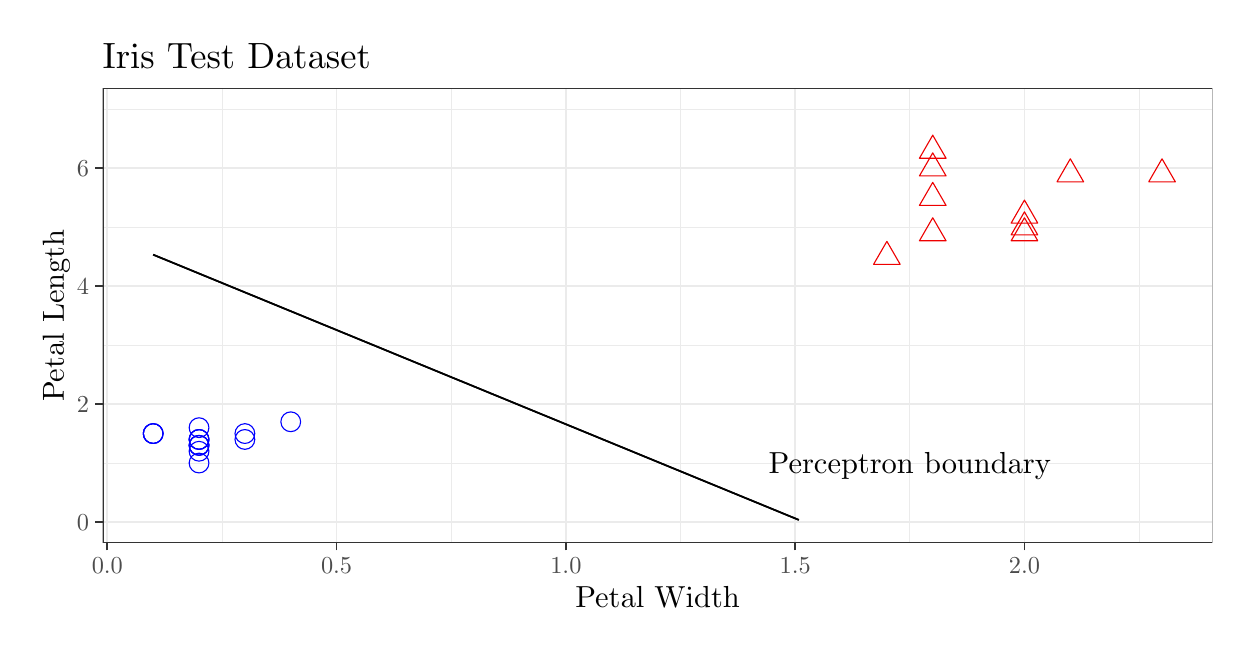
\begin{tikzpicture}[x=1pt,y=1pt]
\definecolor{fillColor}{RGB}{255,255,255}
\path[use as bounding box,fill=fillColor,fill opacity=0.00] (0,0) rectangle (433.62,216.81);
\begin{scope}
\path[clip] (  0.00,  0.00) rectangle (433.62,216.81);
\definecolor{drawColor}{RGB}{255,255,255}
\definecolor{fillColor}{RGB}{255,255,255}

\path[draw=drawColor,line width= 0.6pt,line join=round,line cap=round,fill=fillColor] (  0.00,  0.00) rectangle (433.62,216.81);
\end{scope}
\begin{scope}
\path[clip] ( 27.12, 30.72) rectangle (428.12,194.77);
\definecolor{fillColor}{RGB}{255,255,255}

\path[fill=fillColor] ( 27.12, 30.72) rectangle (428.12,194.77);
\definecolor{drawColor}{gray}{0.92}

\path[draw=drawColor,line width= 0.3pt,line join=round] ( 27.12, 59.49) --
	(428.12, 59.49);

\path[draw=drawColor,line width= 0.3pt,line join=round] ( 27.12,102.10) --
	(428.12,102.10);

\path[draw=drawColor,line width= 0.3pt,line join=round] ( 27.12,144.71) --
	(428.12,144.71);

\path[draw=drawColor,line width= 0.3pt,line join=round] ( 27.12,187.32) --
	(428.12,187.32);

\path[draw=drawColor,line width= 0.3pt,line join=round] ( 70.20, 30.72) --
	( 70.20,194.77);

\path[draw=drawColor,line width= 0.3pt,line join=round] (153.05, 30.72) --
	(153.05,194.77);

\path[draw=drawColor,line width= 0.3pt,line join=round] (235.90, 30.72) --
	(235.90,194.77);

\path[draw=drawColor,line width= 0.3pt,line join=round] (318.76, 30.72) --
	(318.76,194.77);

\path[draw=drawColor,line width= 0.3pt,line join=round] (401.61, 30.72) --
	(401.61,194.77);

\path[draw=drawColor,line width= 0.6pt,line join=round] ( 27.12, 38.18) --
	(428.12, 38.18);

\path[draw=drawColor,line width= 0.6pt,line join=round] ( 27.12, 80.79) --
	(428.12, 80.79);

\path[draw=drawColor,line width= 0.6pt,line join=round] ( 27.12,123.40) --
	(428.12,123.40);

\path[draw=drawColor,line width= 0.6pt,line join=round] ( 27.12,166.01) --
	(428.12,166.01);

\path[draw=drawColor,line width= 0.6pt,line join=round] ( 28.78, 30.72) --
	( 28.78,194.77);

\path[draw=drawColor,line width= 0.6pt,line join=round] (111.63, 30.72) --
	(111.63,194.77);

\path[draw=drawColor,line width= 0.6pt,line join=round] (194.48, 30.72) --
	(194.48,194.77);

\path[draw=drawColor,line width= 0.6pt,line join=round] (277.33, 30.72) --
	(277.33,194.77);

\path[draw=drawColor,line width= 0.6pt,line join=round] (360.18, 30.72) --
	(360.18,194.77);
\definecolor{drawColor}{RGB}{238,0,0}

\path[draw=drawColor,line width= 0.4pt,line join=round,line cap=round] (376.75,169.43) --
	(381.56,161.11) --
	(371.95,161.11) --
	(376.75,169.43);
\definecolor{drawColor}{RGB}{0,0,255}

\path[draw=drawColor,line width= 0.4pt,line join=round,line cap=round] ( 78.49, 68.01) circle (  3.57);
\definecolor{drawColor}{RGB}{238,0,0}

\path[draw=drawColor,line width= 0.4pt,line join=round,line cap=round] (360.18,150.26) --
	(364.99,141.93) --
	(355.38,141.93) --
	(360.18,150.26);

\path[draw=drawColor,line width= 0.4pt,line join=round,line cap=round] (310.47,139.60) --
	(315.28,131.28) --
	(305.66,131.28) --
	(310.47,139.60);
\definecolor{drawColor}{RGB}{0,0,255}

\path[draw=drawColor,line width= 0.4pt,line join=round,line cap=round] ( 61.92, 65.88) circle (  3.57);

\path[draw=drawColor,line width= 0.4pt,line join=round,line cap=round] ( 95.06, 74.40) circle (  3.57);
\definecolor{drawColor}{RGB}{238,0,0}

\path[draw=drawColor,line width= 0.4pt,line join=round,line cap=round] (327.04,171.56) --
	(331.85,163.24) --
	(322.24,163.24) --
	(327.04,171.56);

\path[draw=drawColor,line width= 0.4pt,line join=round,line cap=round] (327.04,148.13) --
	(331.85,139.80) --
	(322.24,139.80) --
	(327.04,148.13);

\path[draw=drawColor,line width= 0.4pt,line join=round,line cap=round] (327.04,177.95) --
	(331.85,169.63) --
	(322.24,169.63) --
	(327.04,177.95);

\path[draw=drawColor,line width= 0.4pt,line join=round,line cap=round] (327.04,160.91) --
	(331.85,152.59) --
	(322.24,152.59) --
	(327.04,160.91);
\definecolor{drawColor}{RGB}{0,0,255}

\path[draw=drawColor,line width= 0.4pt,line join=round,line cap=round] ( 61.92, 63.75) circle (  3.57);

\path[draw=drawColor,line width= 0.4pt,line join=round,line cap=round] ( 45.35, 70.14) circle (  3.57);

\path[draw=drawColor,line width= 0.4pt,line join=round,line cap=round] ( 61.92, 68.01) circle (  3.57);
\definecolor{drawColor}{RGB}{238,0,0}

\path[draw=drawColor,line width= 0.4pt,line join=round,line cap=round] (409.89,169.43) --
	(414.70,161.11) --
	(405.09,161.11) --
	(409.89,169.43);

\path[draw=drawColor,line width= 0.4pt,line join=round,line cap=round] (360.18,154.52) --
	(364.99,146.19) --
	(355.38,146.19) --
	(360.18,154.52);
\definecolor{drawColor}{RGB}{0,0,255}

\path[draw=drawColor,line width= 0.4pt,line join=round,line cap=round] ( 61.92, 65.88) circle (  3.57);

\path[draw=drawColor,line width= 0.4pt,line join=round,line cap=round] ( 78.49, 70.14) circle (  3.57);

\path[draw=drawColor,line width= 0.4pt,line join=round,line cap=round] ( 61.92, 59.49) circle (  3.57);

\path[draw=drawColor,line width= 0.4pt,line join=round,line cap=round] ( 61.92, 72.27) circle (  3.57);

\path[draw=drawColor,line width= 0.4pt,line join=round,line cap=round] ( 61.92, 65.88) circle (  3.57);

\path[draw=drawColor,line width= 0.4pt,line join=round,line cap=round] ( 45.35, 70.14) circle (  3.57);

\path[draw=drawColor,line width= 0.4pt,line join=round,line cap=round] ( 61.92, 68.01) circle (  3.57);

\path[draw=drawColor,line width= 0.4pt,line join=round,line cap=round] ( 61.92, 68.01) circle (  3.57);
\definecolor{drawColor}{RGB}{238,0,0}

\path[draw=drawColor,line width= 0.4pt,line join=round,line cap=round] (360.18,148.13) --
	(364.99,139.80) --
	(355.38,139.80) --
	(360.18,148.13);
\definecolor{drawColor}{RGB}{0,0,255}

\path[draw=drawColor,line width= 0.4pt,line join=round,line cap=round] ( 45.35, 70.14) circle (  3.57);
\definecolor{drawColor}{RGB}{0,0,0}

\path[draw=drawColor,line width= 0.6pt,line join=round] ( 45.35,134.78) --
	( 48.99,133.28) --
	( 52.64,131.79) --
	( 56.28,130.29) --
	( 59.93,128.79) --
	( 63.57,127.29) --
	( 67.22,125.80) --
	( 70.86,124.30) --
	( 74.51,122.80) --
	( 78.16,121.30) --
	( 81.80,119.81) --
	( 85.45,118.31) --
	( 89.09,116.81) --
	( 92.74,115.31) --
	( 96.38,113.82) --
	(100.03,112.32) --
	(103.67,110.82) --
	(107.32,109.32) --
	(110.96,107.83) --
	(114.61,106.33) --
	(118.26,104.83) --
	(121.90,103.33) --
	(125.55,101.84) --
	(129.19,100.34) --
	(132.84, 98.84) --
	(136.48, 97.34) --
	(140.13, 95.84) --
	(143.77, 94.35) --
	(147.42, 92.85) --
	(151.06, 91.35) --
	(154.71, 89.85) --
	(158.36, 88.36) --
	(162.00, 86.86) --
	(165.65, 85.36) --
	(169.29, 83.86) --
	(172.94, 82.37) --
	(176.58, 80.87) --
	(180.23, 79.37) --
	(183.87, 77.87) --
	(187.52, 76.38) --
	(191.16, 74.88) --
	(194.81, 73.38) --
	(198.46, 71.88) --
	(202.10, 70.39) --
	(205.75, 68.89) --
	(209.39, 67.39) --
	(213.04, 65.89) --
	(216.68, 64.40) --
	(220.33, 62.90) --
	(223.97, 61.40) --
	(227.62, 59.90) --
	(231.26, 58.40) --
	(234.91, 56.91) --
	(238.56, 55.41) --
	(242.20, 53.91) --
	(245.85, 52.41) --
	(249.49, 50.92) --
	(253.14, 49.42) --
	(256.78, 47.92) --
	(260.43, 46.42) --
	(264.07, 44.93) --
	(267.72, 43.43) --
	(271.37, 41.93) --
	(275.01, 40.43) --
	(278.66, 38.94);

\path[draw=drawColor,line width= 0.6pt,line join=round] ( 45.35,134.78) --
	( 48.99,133.28) --
	( 52.64,131.79) --
	( 56.28,130.29) --
	( 59.93,128.79) --
	( 63.57,127.29) --
	( 67.22,125.80) --
	( 70.86,124.30) --
	( 74.51,122.80) --
	( 78.16,121.30) --
	( 81.80,119.81) --
	( 85.45,118.31) --
	( 89.09,116.81) --
	( 92.74,115.31) --
	( 96.38,113.82) --
	(100.03,112.32) --
	(103.67,110.82) --
	(107.32,109.32) --
	(110.96,107.83) --
	(114.61,106.33) --
	(118.26,104.83) --
	(121.90,103.33) --
	(125.55,101.84) --
	(129.19,100.34) --
	(132.84, 98.84) --
	(136.48, 97.34) --
	(140.13, 95.84) --
	(143.77, 94.35) --
	(147.42, 92.85) --
	(151.06, 91.35) --
	(154.71, 89.85) --
	(158.36, 88.36) --
	(162.00, 86.86) --
	(165.65, 85.36) --
	(169.29, 83.86) --
	(172.94, 82.37) --
	(176.58, 80.87) --
	(180.23, 79.37) --
	(183.87, 77.87) --
	(187.52, 76.38) --
	(191.16, 74.88) --
	(194.81, 73.38) --
	(198.46, 71.88) --
	(202.10, 70.39) --
	(205.75, 68.89) --
	(209.39, 67.39) --
	(213.04, 65.89) --
	(216.68, 64.40) --
	(220.33, 62.90) --
	(223.97, 61.40) --
	(227.62, 59.90) --
	(231.26, 58.40) --
	(234.91, 56.91) --
	(238.56, 55.41) --
	(242.20, 53.91) --
	(245.85, 52.41) --
	(249.49, 50.92) --
	(253.14, 49.42) --
	(256.78, 47.92) --
	(260.43, 46.42) --
	(264.07, 44.93) --
	(267.72, 43.43) --
	(271.37, 41.93) --
	(275.01, 40.43) --
	(278.66, 38.94);

\node[text=drawColor,anchor=base,inner sep=0pt, outer sep=0pt, scale=  1.10] at (318.76, 55.68) {Perceptron boundary};
\definecolor{drawColor}{gray}{0.20}

\path[draw=drawColor,line width= 0.6pt,line join=round,line cap=round] ( 27.12, 30.72) rectangle (428.12,194.77);
\end{scope}
\begin{scope}
\path[clip] (  0.00,  0.00) rectangle (433.62,216.81);
\definecolor{drawColor}{gray}{0.30}

\node[text=drawColor,anchor=base east,inner sep=0pt, outer sep=0pt, scale=  0.88] at ( 22.17, 35.15) {0};

\node[text=drawColor,anchor=base east,inner sep=0pt, outer sep=0pt, scale=  0.88] at ( 22.17, 77.76) {2};

\node[text=drawColor,anchor=base east,inner sep=0pt, outer sep=0pt, scale=  0.88] at ( 22.17,120.37) {4};

\node[text=drawColor,anchor=base east,inner sep=0pt, outer sep=0pt, scale=  0.88] at ( 22.17,162.98) {6};
\end{scope}
\begin{scope}
\path[clip] (  0.00,  0.00) rectangle (433.62,216.81);
\definecolor{drawColor}{gray}{0.20}

\path[draw=drawColor,line width= 0.6pt,line join=round] ( 24.37, 38.18) --
	( 27.12, 38.18);

\path[draw=drawColor,line width= 0.6pt,line join=round] ( 24.37, 80.79) --
	( 27.12, 80.79);

\path[draw=drawColor,line width= 0.6pt,line join=round] ( 24.37,123.40) --
	( 27.12,123.40);

\path[draw=drawColor,line width= 0.6pt,line join=round] ( 24.37,166.01) --
	( 27.12,166.01);
\end{scope}
\begin{scope}
\path[clip] (  0.00,  0.00) rectangle (433.62,216.81);
\definecolor{drawColor}{gray}{0.20}

\path[draw=drawColor,line width= 0.6pt,line join=round] ( 28.78, 27.97) --
	( 28.78, 30.72);

\path[draw=drawColor,line width= 0.6pt,line join=round] (111.63, 27.97) --
	(111.63, 30.72);

\path[draw=drawColor,line width= 0.6pt,line join=round] (194.48, 27.97) --
	(194.48, 30.72);

\path[draw=drawColor,line width= 0.6pt,line join=round] (277.33, 27.97) --
	(277.33, 30.72);

\path[draw=drawColor,line width= 0.6pt,line join=round] (360.18, 27.97) --
	(360.18, 30.72);
\end{scope}
\begin{scope}
\path[clip] (  0.00,  0.00) rectangle (433.62,216.81);
\definecolor{drawColor}{gray}{0.30}

\node[text=drawColor,anchor=base,inner sep=0pt, outer sep=0pt, scale=  0.88] at ( 28.78, 19.71) {0.0};

\node[text=drawColor,anchor=base,inner sep=0pt, outer sep=0pt, scale=  0.88] at (111.63, 19.71) {0.5};

\node[text=drawColor,anchor=base,inner sep=0pt, outer sep=0pt, scale=  0.88] at (194.48, 19.71) {1.0};

\node[text=drawColor,anchor=base,inner sep=0pt, outer sep=0pt, scale=  0.88] at (277.33, 19.71) {1.5};

\node[text=drawColor,anchor=base,inner sep=0pt, outer sep=0pt, scale=  0.88] at (360.18, 19.71) {2.0};
\end{scope}
\begin{scope}
\path[clip] (  0.00,  0.00) rectangle (433.62,216.81);
\definecolor{drawColor}{RGB}{0,0,0}

\node[text=drawColor,anchor=base,inner sep=0pt, outer sep=0pt, scale=  1.10] at (227.62,  7.44) {Petal Width};
\end{scope}
\begin{scope}
\path[clip] (  0.00,  0.00) rectangle (433.62,216.81);
\definecolor{drawColor}{RGB}{0,0,0}

\node[text=drawColor,rotate= 90.00,anchor=base,inner sep=0pt, outer sep=0pt, scale=  1.10] at ( 13.08,112.75) {Petal Length};
\end{scope}
\begin{scope}
\path[clip] (  0.00,  0.00) rectangle (433.62,216.81);
\definecolor{drawColor}{RGB}{0,0,0}

\node[text=drawColor,anchor=base west,inner sep=0pt, outer sep=0pt, scale=  1.32] at ( 27.12,202.22) {Iris Test Dataset};
\end{scope}
\end{tikzpicture}
